\Section{Numerical results}

\subsection{1D Poisson}

\begin{frame}{Problem considered}
	\textbf{Problem statement:} Consider the Poisson problem in 1D with Dirichlet BC:
	\vspace{-5pt}
	\begin{equation*}
		\left\{
		\begin{aligned}
			-\partial_{xx} u & = f, \; &  & \text{in } \; \Omega \times \mathcal{M},         \\
			u                & =0, \;  &  & \text{on } \; \partial\Omega \times \mathcal{M},
		\end{aligned}
		\right.
	\end{equation*}

	\vspace{-5pt}
	with $\Omega=(0,1)$ and $\mathcal{M}=[0,1]^3$ ($p=3$ parameters).

	\vspace{8pt}
	\textbf{Analytical solution:} $\bm{\mu}=(\mu_1,\mu_2,\mu_3) \in \mathcal{M}$

	\vspace{-5pt}
	\begin{equation*}
		u(x,\bm{\mu})=\mu_1\sin(2\pi x)+\mu_2\sin(4\pi x)+\mu_3\sin(6\pi x).
	\end{equation*}

	\vspace{10pt}
	\textbf{Parametric PINN training:} \\
	MLP 6 layers (sine - 20, 80, 80, 80, 20, 10); Adam optimizer (10000 epochs - 5000 col. pts). \\
	Imposing the Dirichlet BC exactly in the PINN with the levelset $\varphi$ defined by
	\vspace{-8pt}
	$$\varphi(x)=x(x-1).$$

	\vspace{-4pt}
	\textbf{Enriched FEM:} $\mathbb{P}_1$, additive and multiplicative ($M=3$ and $M=100$).
\end{frame}

\begin{frame}{Online phase - 1 parameters instance}
	\setlength{\plotwidth}{0.40\textwidth}\setlength{\plotheight}{0.30\textwidth}
	\vspace{-12pt}
	$$\bm{\mu}=(0.8, 0.5, 0.8) $$

	\begin{minipage}[t]{0.54\linewidth}
		\textbf{Error estimates in $L^2$ norm:}

		{\centering
			\only<1>{\cvgOneDAdd{images/numeric/Poisson1D/cvg}{2}{5e-6}}%
			\only<2->{\cvgOneDAddMult{images/numeric/Poisson1D/cvg}{2}{5e-6}}\par}
	\end{minipage} \hfill
	\begin{minipage}[t]{0.40\linewidth}
		\vspace{8pt}
		\blk{1}{%
			\textbf{Add} $\mathbb{P}_1$: order $2$, as FEM $\mathbb{P}_1$

			\vspace{4pt}
			error $\div\,$\coloredonly<1>{160} vs.\ FEM $\mathbb{P}_1$
		}

		\vspace{12pt}
		\blk*{2}{%
			\textbf{Mult} $\mathbb{P}_1$: order $2$ too

			\vspace{4pt}
			$M=3$: \coloredonly<2>{worse} than Add

			\vspace{4pt}
			$M=100\approx$ Add
		}
	\end{minipage}
\end{frame}

\begin{frame}{Multiplicative versus additive}
	\setlength{\plotwidth}{0.38\textwidth}\setlength{\plotheight}{0.32\textwidth}
	\vspace{-12pt}
	$$\bm{\mu}=(0.3, 0.2, 0.1), \quad \mathbb{P}_1 $$

	\vspace{-4pt}
	\textbf{Gain constants $1/C_\text{gain}$ as a function of $M$:}%\;\refappendix{gain}

	\vspace{4pt}
	\centering
	$L^2$ norm

	\cvgGainConstants{images/numeric/Poisson1D/gain_constants/output_deg0.csv}{1e4}

	\vspace{10pt}
	\uncover<2->{\centering \large \textcolor{darkred}{\textbf{$M\to\infty$: multiplicative $\to$ additive}}\par}
\end{frame}

\subsection{2D Poisson}

\begin{frame}{Problem considered}
	\textbf{Problem statement:} Consider the Poisson problem in 2D with Dirichlet BC:
	\vspace{-5pt}
	\begin{equation*}
		\left\{
		\begin{aligned}
			-\Delta u & = f, \; &  & \text{in } \; \Omega \times \mathcal{M},         \\
			u         & =0, \;  &  & \text{on } \; \partial\Omega \times \mathcal{M},
		\end{aligned}
		\right.
	\end{equation*}

	\vspace{-5pt}
	with $\Omega=(-0.5 \pi, 0.5 \pi)^2$ and $\mathcal{M}=[-0.5,0.5]^2$ ($p=2$ parameters).

	\vspace{8pt}
	\textbf{Analytical solution:} $\bm{\mu}=(\mu_1,\mu_2) \in \mathcal{M}$

	\vspace{-5pt}
	\begin{equation*}
		u(\bm{x},\bm{\mu})=\exp\left(-\frac{(x-\mu_1)^2+(y-\mu_2)^2}{2}\right)\sin(2 x)\sin(2 y).
	\end{equation*}

	\vspace{12pt}
	\textbf{Parametric PINN training:} \\
	MLP 5 layers (sine - 40, 60, 60, 60, 40); Adam then LBFGS optimizer (5000 epochs - 6000 col. pts). \\
	Imposing the Dirichlet BC exactly in the PINN with the levelset $\varphi$ defined by
	$$\varphi(\bm{x})=(x+0.5\pi)(x-0.5\pi)(y+0.5\pi)(y-0.5\pi).$$
\end{frame}

\begin{frame}{Online phase - 1 parameters instance}
	\setlength{\plotwidth}{0.38\textwidth}\setlength{\plotheight}{0.27\textwidth}
	\vspace{-12pt}
	$$\bm{\mu}^{(1)}=(0.05, 0.22) $$

	\begin{minipage}[t]{0.50\linewidth}
		\textbf{Error estimates in $L^2$ norm:}

		{\centering
			\only<1>{\cvgFEMCorrAlldeg{images/numeric/Poisson2D/cvg/FEM_case1_v1_param1.csv}{images/numeric/Poisson2D/cvg/Corr_case1_v1_param1.csv}{1e-10}{false}}%
			\only<2>{\cvgFEMCorrAlldeg{images/numeric/Poisson2D/cvg/FEM_case1_v1_param1.csv}{images/numeric/Poisson2D/cvg/Corr_case1_v1_param1.csv}{1e-10}{true}}\par}
	\end{minipage} \hfill \small
	\begin{minipage}[t]{0.46\linewidth}
		\only<2>{\textbf{$N_\text{dofs}$ required to reach the same error $e$:}

			\vspace{3pt}
			{\centering
				\coststableallq{images/numeric/Poisson2D/costs/TabDoFs_case1_v1_param1.csv}\par}

			$$h\approx N_\text{dofs}^{-1/2}$$
		}
	\end{minipage}

	% \vspace{6pt}
	% \footnotesize Other 2D cases: anisotropic \refappendix{aniso}, annulus with mixed BC \refappendix{annulus}
\end{frame}

\subsection{3D Poisson}

\begin{frame}{Problem considered}
	\textbf{Problem statement:} Consider the Poisson problem in 3D with Dirichlet BC:
	\vspace{-5pt}
	\begin{equation*}
		\left\{
		\begin{aligned}
			-\Delta u & = f, \; &  & \text{in } \; \Omega \times \mathcal{M},         \\
			u         & =0, \;  &  & \text{on } \; \partial\Omega \times \mathcal{M},
		\end{aligned}
		\right.
	\end{equation*}

	\vspace{-5pt}
	with $\Omega=(-0.5 \pi, 0.5 \pi)^3$ and $\mathcal{M}=[-0.5,0.5]^3$ ($p=3$ parameters).

	\vspace{4pt}
	\textbf{Analytical solution:} $\bm{\mu}=(\mu_1,\mu_2,\mu_3) \in \mathcal{M}$

	\vspace{-5pt}
	\begin{equation*}
		u(\bm{x},\bm{\mu})=\exp\left(-\frac{{(x-\mu_1)}^2+{(y-\mu_2)}^2+{(z-\mu_3)}^2}{2}\right)\sin(2x)\sin(2y)\sin(2z).
	\end{equation*}

	\vspace{6pt}
	\textbf{Parametric PINN training:} \\
	MLP 5 layers (tanh - 40, 60, 60, 60, 40); Adam then LBFGS optimizer (5000 epochs - 40000 col. pts). \\
	Imposing the Dirichlet BC exactly in the PINN with the levelset $\varphi$ defined by
	\vspace{-10pt}
	$$\varphi(\bm{x})=(x+0.5\pi)(x-0.5\pi)(y+0.5\pi)(y-0.5\pi)(z+0.5\pi)(z-0.5\pi).$$

	\vspace{-10pt}\small
	Training time: 12 minutes on NVIDIA RTX 2000 (8GB VRAM).
\end{frame}

\begin{frame}{Online phase - 1 parameters instance I}
	\setlength{\plotwidth}{0.37\textwidth}\setlength{\plotheight}{0.30\textwidth}
	\vspace{-12pt}
	$$\bm{\mu}^{(1)}=(0.05, 0.22, 0.1) $$

	\begin{minipage}[t]{0.50\linewidth}
		\textbf{Error estimates in $L^2$ norm:}

		{\centering
			\only<1-2>{\cvgFEMCorrOnedegErr{images/numeric/Poisson3D/cvg/FEM_case1_v2_param1_degree1.csv}{images/numeric/Poisson3D/cvg/Corr_case1_v2_param1_degree1.csv}{2e-5}{false}}%
			\only<3>{\cvgFEMCorrOnedegErr{images/numeric/Poisson3D/cvg/FEM_case1_v2_param1_degree1.csv}{images/numeric/Poisson3D/cvg/Corr_case1_v2_param1_degree1.csv}{2e-5}{true}}\par}
	\end{minipage} \hfill
	\begin{minipage}[t]{0.46\linewidth}
		\only<2-3>{
			\textbf{$L^2$ error w.r.t. online time$^*$:}
			\vspace{4pt}

			{\centering
				\only<2>{\cvgtimeerror{images/numeric/Poisson3D/time_error/FEM_case1_v2_param1_degree1_time_error.csv}{images/numeric/Poisson3D/time_error/Corr_case1_v2_param1_degree1_time_error.csv}{false}}%
				\only<3>{\cvgtimeerror{images/numeric/Poisson3D/time_error/FEM_case1_v2_param1_degree1_time_error.csv}{images/numeric/Poisson3D/time_error/Corr_case1_v2_param1_degree1_time_error.csv}{true}}\par}
			\vspace{-4pt}

			\footnotesize
			$^*$ mesh + assembly + solve \\
			\textcolor{addcolor}{\; + prior derivatives evaluation} \\
			\textcolor{addcolor}{\; \sout{+ training time}}
		}
	\end{minipage}
\end{frame}

\begin{frame}{Online phase - 1 parameters instance II}
	\vspace{-12pt}
	$$\bm{\mu}^{(1)}=(0.05, 0.22, 0.1) $$

	\textbf{$N_\text{dofs}$ and online time required to reach the same error $e$:}

	\begin{table}[ht!]
		\centering
		\timerequired{images/numeric/Poisson3D/timerequired/TabTimes_case1_v2_param1_degree1.csv}
	\end{table}
	\hspace{240pt}\begin{tikzpicture}
		\flechecourbehorizontale{2.5}{0.1}{2}{-0.2}{$\div 1471$}{darkred}
	\end{tikzpicture}

	\begin{minipage}[t]{0.6\linewidth}
		Cartesian mesh: $N_\text{dofs} = N^3$ nodes ($\mathbb{P}_1$ elements).

		\vspace{10pt}
		\footnotesize
		$^*$ The results in brackets are extrapolations.
	\end{minipage} \hfill \begin{minipage}[t]{0.35\linewidth}
		\centering

		\vspace{15pt}
		\Large
		\only<2>{\textcolor{darkred}{\warning Training time !}}
	\end{minipage}
\end{frame}

\begin{frame}{Parametric framework}
	\setlength{\plotwidth}{0.38\textwidth}\setlength{\plotheight}{0.27\textwidth}
	\textbf{How many parameters instance $n_p$ are needed to balance training?}

	\vspace{-5pt}
	\begin{minipage}[t]{0.48\linewidth}
		\centering
		\cvgtimeerrorparam{images/numeric/Poisson3D/parametric_framework/output13.csv}

		\vspace{-4pt}
		To achieve $e=10^{-3}$
	\end{minipage} \hfill
	\begin{minipage}[t]{0.48\linewidth}
		\centering
		\cvgtimeerrorparamD{images/numeric/Poisson3D/parametric_framework/output54.csv}

		\vspace{-4pt}
		To achieve $e=5\cdot 10^{-4}$
	\end{minipage}

	\vspace{10pt}
	\textbf{Online:} assembly + solve \textcolor{addcolor}{\; + prior derivatives evaluation} \\

	\textbf{Offline:} mesh	\textcolor{addcolor}{\; + training time}
\end{frame}
